\section{Corpus Task Complexity}

\begin{figure}[t]
    \centering
    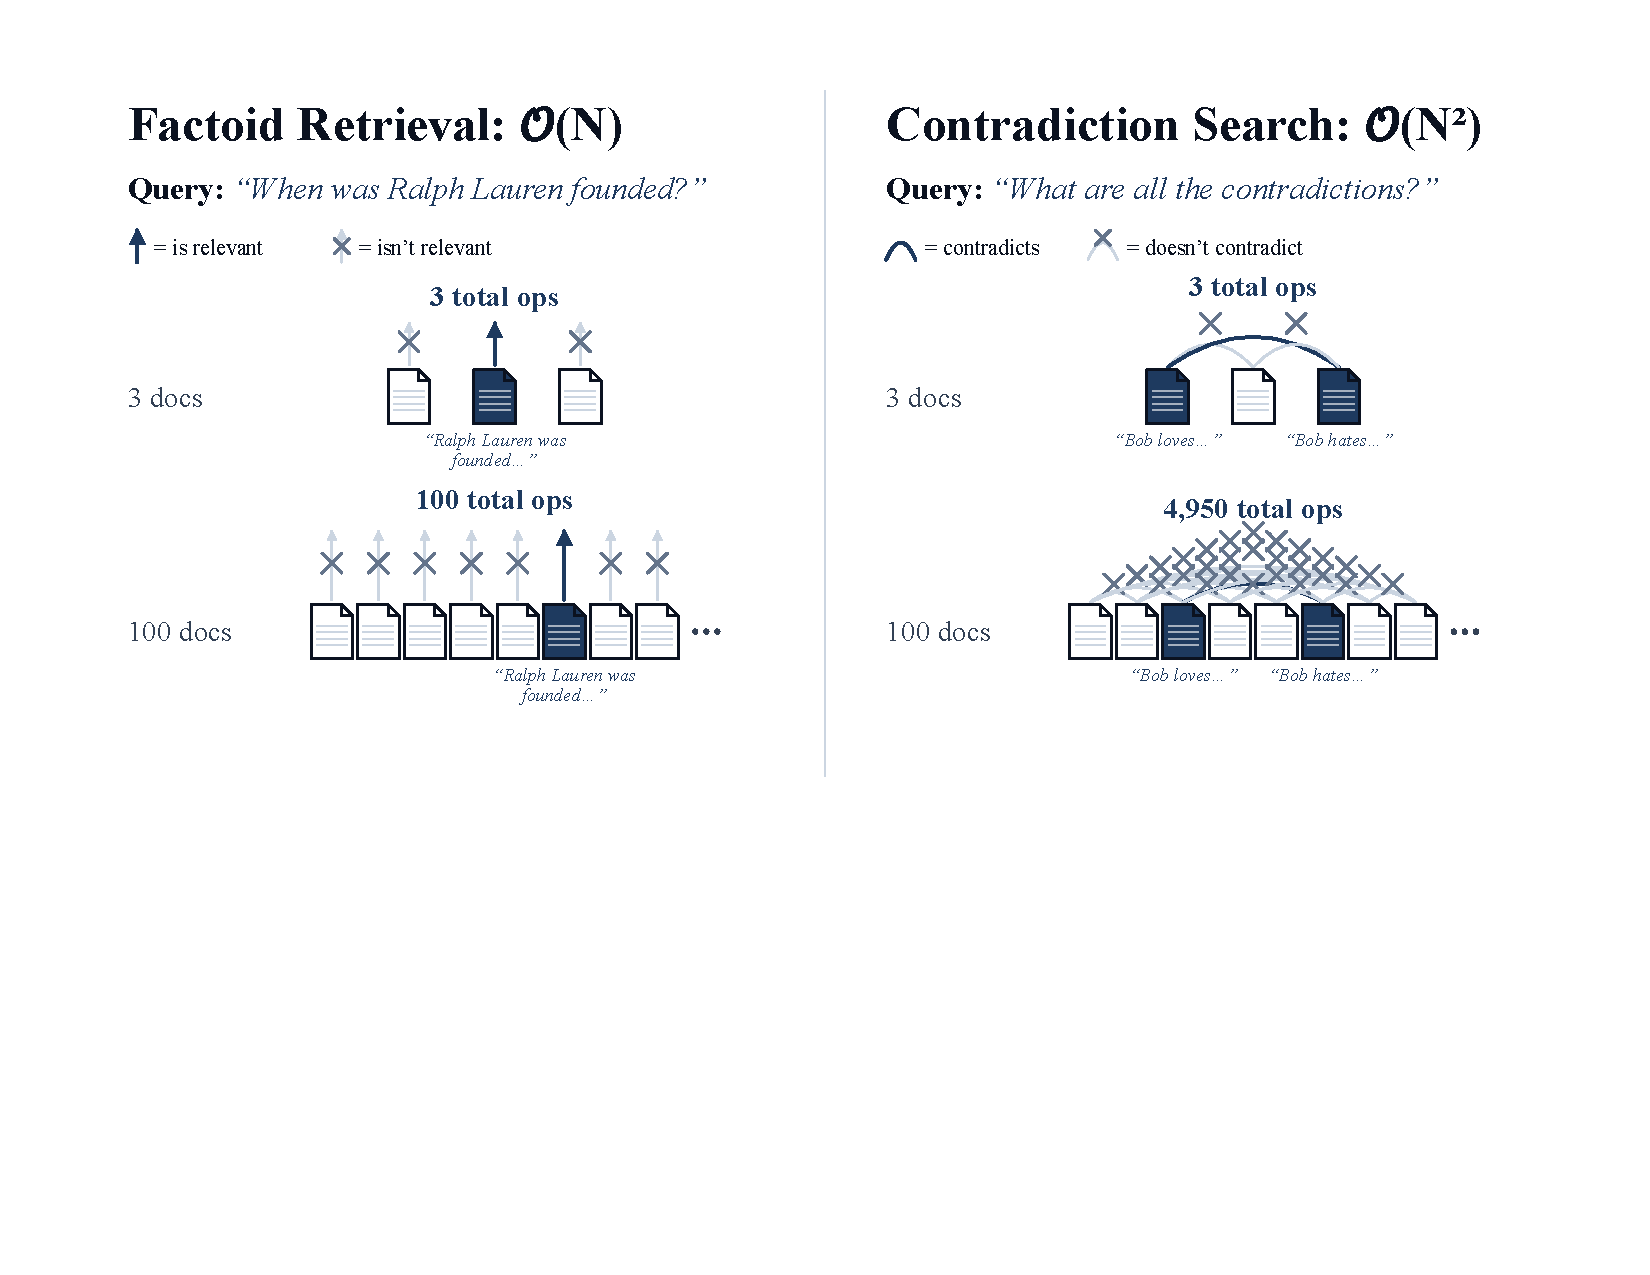
\includegraphics[width=\textwidth, trim= 60 270 60 0]{figures/Figure 1 — Print.pdf}\\
    \caption{ (Right) As corpus grows, a contradiction search task requires many more basic operations (4950) than factoid retrieval (100). \prasann{update with pubmed exapmle}}
    \label{fig:ctcexplanation}
\end{figure}


% \prasannnote{todo get a good figure}

Our corpus task complexity definition is central to the rest of this work. We here define it, connect it to existing work, and then use it to identify and propose a new class of tasks. 

% \jsnote{Suggested restructure: ``''}
% Corpus reasoning is a blanket term for tasks over large corpora. We define a corpus as a set of N documents $d_1, . . . , d_N \in C$. A corpus reasoning query $q$ is simply a query which requires synthesizing and analyzing information within or across documents.  Prior work has heavily studied various such tasks, but our unified framework helps explain what makes certain tasks more challenging and encourages the community to shift beyond \ctc{N} tasks. We concretize this below:

% \amandanote{what trends?}

% \sewonnote{I think this section is overall very strong. Suggestion: I think we should write this section to be a bit more broad and not tied to specific tasks/datasets we are testing such as NQ, e.g., moving the last paragraph of Section 2.1 to somewhere else, and moving Section 2.3 to somewhere else.
% (UPDATE) After reading Section 2.3, I think a better solution might be that we keep Section 2.3, but frame it as a list of tasks we consider and describe it in a domain/data-agnostic way, e.g., by describing it as a general task 'type'. Then, a later section can specify how each task is instantiated in practice, e.g., using NQ, etc. Overall, Section 2 does not need to mention specific dataset names/domain names and can stay fully general.}\sewonnote{Also I think  the novelty of Section 2.2 can come across as stronger, e.g., could we rename the subsection title to CTC, and clearly frame in the main text that we are defining this new metric?} \prasannnote{I tried to address, not sure if better?}

% \subsection{Task Definition }
% \label{sec:task-def}


\subsection{Corpus Task Complexity}
% ⚠ THIS IS THE ONLY \label{sec:definitioncomp}. There were two, and BOTH were misplaced: one sat
% just after \end{figure} (so it anchored to figure.2, not a section) and one sat just BEFORE
% \subsection{Connecting Common Tasks...} (a \label binds to the last counter STEPPED, so it took
% the preceding subsection). The refs all mean "the subsection where CTC is defined", which is this
% one, and it still renders as 2.1 -- the number does not change, only what it points at.
\label{sec:definitioncomp}
% \sewonnote{First of all, I think this section is going to the right direction: defining complexity as a function of the task rather than the model, and grounding it in a clear functional formulation!
% Suggestion: how about we define the atomic interaction as a pairwise interaction (either between query-document, or document-document), and define task complexity as the number of atomic interactions required to perform the task? I think that's kind of how your paragraph is describing already, but currently the definition of atomic operation isnt' pairwise.} 
% \prasannnote{Tried sewon's suggestion out. It's a bit simpler though I guess formally less clean / general?}

% \sewonnote{Suggested opening (just a flow; language should be refined): ``We have vague sense on which tasks are more complex/simpler than other, but how can we concretely quantify task complexity? To this end, we define corpus task complexity (CTC), which is based on how the required computation scale as the corpus size N grows. Specifically, we first define atomic operation...., and then quantify how many such atomic operations is needed to perform the task.''}

% \prasannnote{Try jacob idea of language oracle that can work with O(1) length input and O(1) question and outputs an answer.}

% \jsnote{Suggested re-write: ``To help taxonomize corpus reasoning tasks by their difficulty, we introduce a heuristic notion of complexity that we call \emph{corpus task complexity}. Specifically, imagine we have access to a natural language oracle that can take in $O(1)$-length contexts and $O(1)$-length questions and outputs an answer (for instance, an LM-judge with fixed context length). The corpus task complexity (CTC) is the number of operations needed to solve a task as a function of the corpus size (and potentially other parameters).

% As an example, for a query .... ''}
Define a corpus $C$ to be a set of $N$ documents $\{d_1, \ldots, d_N\}$, where each $d_i$ is a sequence of tokens. A corpus reasoning task is a dataset of question-answer samples $(q_i, a_i)$ about corpus $C$. For instance, for factoid question answering, a sample could be could be $C=$ Wikipedia, $q_i=$\emph{``Who was the US president in 1967?''}, and $a_i$=\emph{``Lyndon Johnson''}. For a contradiction search task $q_i$ is \emph{``What are all the contradictions?''}, with $a_i$ depending on the corpus (e.g. [(``\emph{15 studies indicate a protective effect of cigarette smoking...}'', ``\emph{cigarette smoking is linked to renal cancer}'')]). 

To understand corpus reasoning task requirements, we define a heuristic notion of complexity called \emph{corpus task complexity}. Specifically, imagine that we have access to a natural language oracle that can take in $O(1)$-length contexts and $O(1)$-length questions and outputs an answer (for instance, an LM-judge with fixed context length). The corpus task complexity (CTC) is the order of oracle operations needed to solve tasks as a function of corpus size $N$. \cname, defined at the task level, is identifiable independent of methods (LCLMs, dense retrieval, etc.), but we posit that it corresponds to real computational requirements of models to handle tasks, especially as corpus scale grows.  

\textbf{Example 1: }For a 100 document corpus and query $q =$ \emph{``When was Ralph Lauren founded?''} (Figure~\ref{fig:ctcexplanation}, left), an oracle operation is $\mathrm{isrelevant}(d_i, q)$: whether a given document $d_i$ is relevant to the query $q$. In this case, for the entire corpus, we'd need $N=100$ operations to check \emph{every} document, hence we can say this is $O(N)$ operations in the number of documents, or \ctc{N} (we use blue and $T$ to indicate \emph{task} complexity). 

\textbf{Example 2:} For another 100 document corpus (Figure~\ref{fig:ctcexplanation}, right), with sentence documents, given the query $q =$ \emph{``Find all contradicting sentences''}, the oracle operation is $\mathrm{contradicts}(d_i, d_j)$: whether sentences $i$ and $j$ contradict. In this cases, for the entire corpus, we'd need $N=4,950$ oracle operations to check every possible pair, which is \ctc{N^2} in corpus size. Note how this scales much faster at larger corpus sizes than the previous example.

Complexity of tasks can be diverse, from \ctc{1} tasks (e.g. common knowledge questions like ``What's the capital of India'' likely don't require looking at the corpus), to \ctc{N^3}, and especially on larger corpora, we expect \cname to play a dominant role. That said, while \cname assumes constant average oracle operation cost, tasks with harder oracle operations---even within CTC---will be more challenging, and atomic task difficulty likely compounds at higher complexities.  \prasannnote{Wrote this paragraph for reviewer concerns}

% \prasann{Acknowledge Assumptions and address simplicity concerns, then just skip to data descriptions and talk about more task complexities there}

% One may have a rough sense of which tasks are more complex than others, but \emph{how can we concretely quantify task complexity}? To this end, \textbf{we propose the framework of corpus task complexity (CTC)}, based on how required computation scales alongside corpus size N. We first define \emph{atomic operations}, and then quantify how many such atomic operations are needed to perform a task.

% ---either query-document ($a(q, d_{i})$; \emph{``does the chunk contain the answer to the question?''}) or between documents ()...., and then quantify how many such atomic operations is needed to perform the task. \prasann{overloading }

% Given an initial document $d_i$, we define a pairwise \textbf{atomic operation} as an interaction between (i) $d_i$ and a query $q$ (e.g. \emph{``is this document relevant to the question?''}) or (ii) between $d_i$ and another document $d_j$ (e.g.  \emph{``are these 2 documents conflicting?''}). Concretely we write this as $a(d_{i}, q)$ or $a(d_{i}, d_{j})$ respectively, where $a$ has a roughly constant \emph{computational cost}  $c(a)$ across inputs. 

% Corpus reasoning queries can be decomposed into series of atomic interactions over the corpus. For example, given query $q =$ \emph{``Which outputs show sycophantic behavior?''}, we can answer $q$ over the corpus by simply running some aggregation $\sum_{i=1}^N(a(q, d_i))$: checking one document at a time to see if it's relevant or not. In this example, the \emph{total computational cost} is around $N * c(a)$, thus its \textbf{corpus task complexity} is \ctc{N} (we color this blue and include the subscript to distinguish task complexity from method computational complexity). 

% \cname is simply an abstract framework to reason over the kinds of operations needed to handle a corpus reasoning task over increasing $N$, and which models may need to do internally in some capacity. We'll investigate 3 \cname types. \prasannnote{state more obviously}

% {\boldmath \ctc{N}:} If a task can be broken into oracle operations based on single or neighboring documents at a time, it's likely \ctc{N}. The ``sycophantic behavior'' query from the previous paragraph is one example, but book summarization (individual or neighboring passages can be summarized independently then concatenated) could be another. Multi-hop QA, which can be broken into a constant number of \ctc{N} retrieval steps, will also be \ctc{N}. Interestingly, we note that most prior corpus reasoning tends to focus on \ctc{N} tasks \citep{Bertsch2025OolongEL, Yen2024HELMETHT, Chen2026LongBenchPA, Bai2024LongBenchVT, Yang2018HotpotQAAD, izacardNQ}.


% % \sewonnote{I think having each paragraph to have a concrete running example, and how exactly that is either \ctc{N}, \ctc{N^2}, etc, would be nice.}

% {\boldmath \ctc{N^2}:} If a task involves oracle operations that identify pairwise relationships between arbitrary documents (e.g. \emph{``A contradicts B'', ``A follows from B''...}), this is likely \ctc{N^2}. The contradiction task we use throughout (recall Figure~\ref{fig:motivatingtask}) is one example. This is because, assuming all possible pairs are plausible, exhaustively checking every possible pair (i.e. a nested for loop) is \ctc{N^2}.  % \amandanote{the oolong-pairs dataset from the RLMs paper might fall under this, would need to check the details again to be sure}

% {\boldmath \ctc{NM}:} Sometimes, \cname may depend on factors other than $N$. For example, for unsupervised clustering or organization style tasks, a naive algorithm to handle such a task is for the oracle to check if pairs of documents are in existing clusters---if not, the document can be added to a new cluster. Assuming $M$ total clusters, this would involve \ctc{NM} comparisons. 

% By separating higher \cname tasks from commonly studied \ctc{N} tasks, we can more clearly identify their differing evaluation and methodological needs.



\subsection{Connecting Common Tasks to \cname}
% ---------------------------------------------------------------------------
% Preamble requirements:  \usepackage{booktabs,multirow,tabularx,array}
% If your paper is two-column, change table -> table* (both \begin and \end):
% the table is ~1.2 pages tall inside a single column, and a float that does
% not fit on a page is silently deferred and never printed.
% ---------------------------------------------------------------------------
% Fallbacks in case \ctc / \cname are not already defined in your preamble.
% \ensuremath is what lets you write \ctc{N^2} without a "Missing $ inserted" error.
\providecommand{\ctc}[1]{\ensuremath{\mathcal{O}_T(#1)}}
\providecommand{\cname}{CTC}

% ---------------------------------------------------------------------------
% Preamble requirements:  \usepackage{booktabs,multirow,array}
% If your paper is two-column, change table -> table* (both \begin and \end):
% the table is ~1.2 pages tall inside a single column, and a float that does
% not fit on a page is silently deferred and never printed.
% ---------------------------------------------------------------------------
% Fallbacks in case \ctc / \cname are not already defined in your preamble.
% No tabularx: column widths are fractions of \linewidth, so it still auto-fits.
% \ensuremath is what lets you write \ctc{N^2} without a "Missing $ inserted" error.
\providecommand{\ctc}[1]{\ensuremath{\mathcal{O}_T(#1)}}
\providecommand{\cname}{CTC}
\ifdefined\catw\else\newlength{\catw}\newlength{\dsw}\newlength{\metw}\newlength{\descw}\fi

% Preamble requirements:  \usepackage{booktabs,array}
% If your paper is two-column, change table -> table* (both \begin and \end).
\providecommand{\ctc}[1]{\ensuremath{\mathcal{O}_T(#1)}}
\providecommand{\cname}{CTC}
\ifdefined\catw\else\newlength{\catw}\newlength{\dsw}\newlength{\metw}\newlength{\descw}\fi




% Preamble:  \usepackage{booktabs,array}
% Use table* in a two-column paper -- each panel gets only half the given width.
\providecommand{\ctc}[1]{\ensuremath{\mathcal{O}_T(#1)}}
\providecommand{\cname}{CTC}
\ifdefined\catw\else\newlength{\catw}\newlength{\dsw}\newlength{\metw}\newlength{\descw}\fi

\newcommand{\panelcols}{%
  \setlength{\catw}{\dimexpr0.27\linewidth-2\tabcolsep\relax}%
  \setlength{\dsw}{\dimexpr0.33\linewidth-2\tabcolsep\relax}%
  \setlength{\descw}{\dimexpr0.40\linewidth-2\tabcolsep\relax}%
}
\newcommand{\blk}[1]{\multicolumn{3}{@{}l}{#1} \\}
\providecommand{\ex}[2]{#1~$\rightarrow$~\texttt{#2}}

\begin{table}[t]
\centering
\scriptsize
\setlength{\tabcolsep}{4pt}
\renewcommand{\arraystretch}{1.12}

\begin{tabular}{@{}
  >{\raggedright\arraybackslash}p{0.18\linewidth}
  >{\raggedright\arraybackslash}p{0.29\linewidth}
  >{\raggedright\arraybackslash}p{0.18\linewidth}
  >{\raggedright\arraybackslash}p{0.29\linewidth}
@{}}
\toprule
\multicolumn{2}{c}{\textbf{\(\mathbf{O}(N)\): One-pass tasks}} &
\multicolumn{2}{c}{\textbf{Higher-complexity tasks}} \\
\cmidrule(r){1-2}\cmidrule(l){3-4}
\textbf{Dataset} & \textbf{Description} &
\textbf{Dataset} & \textbf{Description} \\
\midrule

NQ
  & Retrieve the answer passage
  & Outlier (wiki, scale-\(k\))
  & Find chunks from the rarest article \\

HotpotQA (bridge)
  & Retrieve two supporting passages
  & Grouping (OpenAlex)
  & Group abstracts by a latent topic \\

NIAH-contra
  & Find the contradicting claim
  & Contradiction
  & Find all contradicting claim pairs \\

BEIR SciFact
  & Retrieve evidence for a scientific claim
  & xabsence
  & Find unmatched docs across 2 shuffled, near-identical corpora \\

BEIR FiQA
  & Retrieve relevant financial opinions
  & strmatch
  & Find pairs sharing a word sequence \\

MS MARCO
  & Retrieve relevant web passages
  & qdmatch (NQ)
  & Match questions to documents \\

MS MARCO rerank
  & Re-rank passages by relevance
  & qdmatch (HPQA)
  & Match questions to two documents \\

OBLIQ
  & Retrieve passages for subjective queries
  & qdmatch (FiQA)
  & Match financial queries to documents \\

Oolong
  & Aggregate labels over the corpus
  & Reorder
  & Recover the order of shuffled segments \\

Outlier (Amazon)
  & Find reviews with the minority attribute
  & Textgroups
  & Find passage triples satisfying a target \\

Outlier (wiki, fixed \(M\))
  & Find items from the rarest article
  & & \\

Absence
  & Identify content missing from a copy
  & & \\

\bottomrule
\end{tabular}

\caption{\textbf{Overview of the 22 \bench{} Tasks.}
Linear-time tasks are shown on the left; tasks requiring
category-wise, pairwise, or higher-order comparisons are shown on the right.
Appendix~\ref{app:examples} provides an example of each task.
}
\label{tab:eval-datasets}
\end{table}

\prasann{Cite everything} How do existing corpus reasoning tasks factor into \cname? \emph{Information retrieval (IR)}, a highly studied example, where the task is to find documents relevant to some query, is \ctc{N} as queries only need to see documents constant numbers of times. We include several standard IR settings, such as MS-MARCO, BEIR tasks (SciFact, FiQA), representing a spectrum of retrieval difficulties. As a more modern inclusion, we include the twitter set of OBLiQ (CITE), a challenging recent abstract retrieval setting. 

Beyond IR, LCLM literature has focused on its own standard suite of tasks, represented in benchmarks like LongBenchv2 or HELMET. Most common is \emph{Factoid Question Answering}---which answers questions given a corpus---and is also \ctc{N} like retrieval as they are typically decomposable into finding 1 or 2 chunks relevant to queries. \emph{NaturalQuestions} and \emph{HotpotQA} (a multi-hop QA setting, which given constant hops is still \ctc{N}) are popular examples. \emph{Documenting re-ranking}, which involves finding the top-k most relevant documents to search queries, is also common, and as k is typically much smaller than corpus size, is \ctc{N}, also decomposing into retrieval.

Less common but also studied with LCLMs more recently are \emph{Aggregation} settings, for example OOLONG, which involves answering distributional or counting questions about the class labels of corpora. We further include an Amazon based outlier setting that requires finding chunks from the least common product category or topics. Note that this decomposes to \ctc{N}, as given fixed class types it's possible to make a single pass to get individual document labels to aggregate. \emph{Corpus Edit} settings, like AbsenceBench, which search for differences in near-identical corpora, are \emph{also} \ctc{N}, as it's possible to simply track whether chunks at fixed positions in corpora match.

% We start with a diverse group of tasks which we posit can be reduced to an order of $N$ oracle operations. As a well-studied task, we include a variety of \emph{retrieval settings} (given a query, output the document ids of the relevant documents), where the oracle operation is whether a document is relevant to the query. Our suite varies from easier settings like \textbf{MSMARCO, FiQA, SciFact, NQ} based on the BEIR retrieval suite \prasann{TODO cite}, to a multi-hop retrieval setting based on \textbf{HotpotQA} (retrieve 2 documents which combine to answer the query), to the challenging modern \textbf{OBLiQ} \prasann{TODO cite} retrieval set with highly abstract queries from the paper's twitter set. As a direct comparison to our high-\cname contradiction setting we also include a \textbf{contradiction needle-in-a-haystack} (NIAH) setting where given a pubmed claim sentence the model needs to find the almost word-matched contradicting claim in the corpus. We mine BM25 based hard-negatives from source corpora for all of these to up to 10\% corpus size (except for contradiction NIAH).

% Several other \ctc{N} settings include \emph{fixed class aggregation settings} like \textbf{Amazon Outliers}, where the task is to find the least common category from a small set of product categories (shared across train / test set) in a corpus of reviews, or \textbf{OOLONG}, which focuses on computing which chunk classes are most common or have certain properties. The atomic operation in these involves labeling each chunk with a predefined class, and potentially tracking a small amount of global state (e.g. which classes are most common from prior operations) with each operation. An \emph{exact diff} setting like \textbf{gutenberg absence} (given 2 project gutenberg book passages with a few deleted sentences, find the deleted sentence ids), a cross-corpus task where an atomic operation is to just check the corresponding fixed index at an offset also only requires roughly $N$ oracle operations. We lastly include a \textbf{NarrativeQA} setting (answer an extractive question about a book), similar to a retrieval setting, and a \textbf{govreport summarization} setting where an atomic operation is to synthesize a chunk of text into compressed content. 

\subsection{\bench{} and High \cname Tasks}

The above tasks constitute a recent, diverse, and representative sample of corpus reasoning tasks studied in retrieval and LCLM literature, yet strikingly, \textbf{they all fall into \ctc{N}}. Our definition of \cname suggests that a variety of useful tasks should fall into higher complexity classes, yet such tasks, while touched on at small scale (e.g. event re-ordering CITE, LongBenchV2 cite), are understudied for larger corpora, especially in the context of LCLMs. We thus, to enable our analysis, construct a diverse suite of 10 \cname tasks. While partially synthetic for controllability and cleaner analysis, \bench{} structurally represent various realistic tasks with diverse \cname{}.  We'll call these tasks---along with our collected low \cname tasks---\bench{} (Table~\ref{tab:eval-datasets}):

\emph{Contradiction}, which plants LLM-generated contradictions to pubmed abstract claims, is as discussed earlier \ctc{N^2} (Example 2, Section~\ref{sec:definitioncomp}). So is \emph{X-Absence}, which, reminiscent of work comparing differences in text distributions (cite), aims to find the documents not shared between two near-identical corpora---the atomic operation is whether two documents are the same, but across corpora. To compare more closely against retrieval settings, and further study cross-corpus comparison, we include 3 query-document matching \emph{(QDmatch)} settings, where across two same-sized corpora---one of random queries and one of documents---one must find the 3 query-document pairs that match---these are also \ctc{N^2} similar to X-Absence.

\cname isn't always necessarily a factor of $N$. Our wikipedia outlier setting, which shuffles chunks from $M$ pages, requires identifying the chunks belonging to the least commonly featured page. Unlike OOLONG, which has fixed classes, possible classes (source page topics) are too large, and so this requires cross-chunk comparison, but given an atomic operation of $\mathrm{samecategory(d_i, d_j)}$, one exemplar per category is enough to figure out groups, thus making the task \ctc{NM}. To test this categorization we include a setting where $M$ stays constant and one where $M$ grows proportional to $N$. We include a grouping task which dynamically must group abstracts, and is also \ctc{NM}.

% ⚠ MOVED, NOT EDITED (no words changed). This wraptable opened mid-sentence, appended to the end
% of the preceding paragraph's last line. wrapfig requires a paragraph boundary; from inside a
% paragraph it cannot reserve the column and falls back to floating.
\begin{wraptable}{r}{0.4\textwidth}
\centering
\small
\setlength{\tabcolsep}{5pt}
\begin{tabular}{lrr}
\toprule
Task & No Mix & Mix \\
\midrule
BEIR FiQA & 0.648 & \textbf{0.658} \\
Outlier (scale-$k$) & 0.083 & \textbf{0.588} \\
QDmatch (FiQA) & 0.212 & \textbf{0.243} \\
Reordering & 0.000 & \textbf{0.182} \\
Contradiction & 0.000 & \textbf{0.791} \\
\bottomrule
\end{tabular}
\caption{Our curriculum mask-mixing trick helps chunk attention across settings, especially high-\cname settings}
\label{tab:maskmix}
\end{wraptable}

Lastly we include some more challenging (albeit synthetic) tasks---for example an \ctc{N^2} \emph{Strmatch} setting to find pairs of word sequences sharing long enough common substrings, and a \emph{re-order} task (\cite{Bai2024LongBenchVT}) which requires sorting shuffled book passages, also $N^2$ with an oracle operation of $\mathrm{directlyneighbours(d_i, d_j)}$, requiring a brute-force sort. Lastly, we include the \ctc{N^3} Textgroups setting which looks for document triples which combine to have the right properties (e.g. 71 total nouns). 

% We include several other tasks as well. For example several tasks we classify as \ctc{NM}, where other variables may determine scaling behavior. We include three \textbf{qdmatch settings}, directly comparable to corresponding retrieval settings (OBLiQ, HPQA, NQ) where the corpus contains a mixture of queries and documents, and the task is, given exactly 3 matching query document pairs, find the relevant pairs. Here the atomic operations are only relevance judgements between queries $M$ and documents $N$. This similarly applies to our \textbf{random absence} setting which checks to see given 2 random shuffled, near identical corpora, which documents in corpus B \emph{aren't} in corpus A, or vice-versa. Our \textbf{outlier} setting, which involves finding, given a set of $N$ chunks sampled from $M$ multi-chunk wikipedia documents (we treat this as a topical group), which chunks come from the least common ``group'' is also \ctc{NM}, where the oracle operation is determining whether a document fits into an existing group, and scales by the number of groups. The \textbf{grouping} setting, which groups a full corpus of OpenAlex (TODO cite) abstracts at different levels of granularity is similar.

% We lastly, for reference, include a synthetic \ctc{N^3} \textbf{textgroups} setting which, given some textual feature (e.g. how many nouns, how many times a word occurs, etc.), looks for groups of 3 chunks which total to have the same value. 

% Note that many of these tasks are somewhat synthetic. This is in part due to the scarcity of existing, scalable high-CTC benchmarks for LCLMs, and in part to enable greater control and clearer analysis (which is the focus of this work). The creation of realistic high-\cname corpus reasoning benchmarks are an exciting future direction, but would be a large additional undertaking orthogonal to this work, and would likely be too difficult to analyze clearly even at small scale. That said, we model our tasks to structurally resemble a variety of high-CTC tasks we believe to be realistic, and are a useful first step to analysis and evaluation of these problems. To support larger-scale research \emph{we \prasann{TODO} release eval sets up to 10M token context lengths on our settings}. \prasannnote{I don't think we need a section for eval sets, I think this line is enough.} \prasannnote{more for project w amanda but I think we can use single corpus / swap queries, last part of context to reduce eval times}

% \begin{table}[t]
% \centering
% \small
% \setlength{\tabcolsep}{4pt}
% \renewcommand{\arraystretch}{1.05}
% \begin{tabular}{@{}l l p{5.4cm} l@{}}
% \toprule
% \textbf{Task} & \textbf{Documents} & \textbf{Oracle operation} & \textbf{Metric} \\
% \midrule
% \multicolumn{4}{@{}l}{\textbf{\ctc{N}} --- one pass over the corpus} \\
% \midrule
% NQ                  & Wikipedia 100w    & does $d_i$ answer $q$?                              & gold-ID F1 \\
% HotpotQA (bridge)   & Wikipedia 100w    & does $d_i$ support one hop of $q$?                  & gold-ID F1 \\
% NIAH-contra         & PubMed claims     & does $d_i$ contradict the query claim?              & set-F1 \\
% BEIR SciFact        & science abstracts & does $d_i$ bear on claim $q$?                       & set-F1 \\
% BEIR FiQA           & finance posts     & does $d_i$ answer $q$?                              & set-F1 \\
% MS MARCO            & web passages      & does $d_i$ answer $q$?                              & set-F1 \\
% MS MARCO rerank     & web passages      & how relevant is $d_i$ to $q$?                       & MRR@10 \\
% OBLIQ               & posts / abstracts & does $d_i$ match $q$'s subjective criterion?   & set-F1 \\
% Oolong              & labeled items     & what is item $i$'s label? (then aggregate)    & partial credit \\
% NarrativeQA         & books, scripts    & (single document; long-context QA)                  & token-F1 \\
% GovReport           & gov.\ reports     & (single document; summarization)       & ROUGE \prasann{WIP} \\
% \midrule
% \multicolumn{4}{@{}l}{\textbf{\ctc{NM}} --- categorization, $M$ inferred from the corpus} \\
% \midrule
% Outlier (wiki)      & Wikipedia 100w    & which article does $d_i$ belong to?                 & set-F1 \\
% Grouping            & OpenAlex abstracts& is $d_i$ in the same subfield as cluster $m$?       & pairwise-F1 / ARI \\
% \midrule
% \multicolumn{4}{@{}l}{\textbf{\ctc{N^2}} --- all-pairs search} \\
% \midrule
% Contradiction       & PubMed claims     & do $d_i$ and $d_j$ contradict?                      & pair-F1 / EM \\
% Absence             & Gutenberg       & is $d_i$ present in version 2?             & set-F1 \\
% xabsence            & PubMed claims     & does some $d_j \in B$ paraphrase $d_i \in A$?     & set-F1 \\
% strmatch            & word strings      & do $d_i, d_j$ share a $k$-word run?                 & pair-F1 \\
% qdmatch (NQ)        & Wikipedia 100w    & does document $d_j$ answer query $q_i$?             & pair-F1 \\
% qdmatch (HPQA)      & Wikipedia 100w    & \dots{}with two gold documents per query             & pair-F1 \\
% qdmatch (OBLIQ)     & long abstracts    & \dots{}with long queries and documents               & pair-F1 \\
% Reorder             & Gutenberg         & does $d_i$ precede $d_j$?                           & Kendall-$\tau$ \\
% \midrule
% \multicolumn{4}{@{}l}{\textbf{\ctc{N^3}} and beyond --- groups, not pairs} \\
% \midrule
% Cycle               & comparison claims & do $d_i, d_j, d_k$ close a ranking loop?            & group-F1 \\
% Groups-of-4         & expressions       & are 4 values mutually within $X$?                   & group-F1 \\
% Textgroups          & short passages    & do 3 passages' feature counts sum to $T$?           & group-F1 \\
% \bottomrule
% \end{tabular}
% \caption{\textbf{The corpus-reasoning task suite (24 tasks).} Each row gives the document source, the atomic oracle operation the task decomposes into (Section~\ref{sec:definitioncomp}), and the metric. \cname{} is determined by how many such operations are required as $N$ grows: one per document (\ctc{N}), one per document-category pair (\ctc{NM}), one per document pair (\ctc{N^2}), or one per group (\ctc{N^3}). Roughly half are ports of published benchmarks and half are constructed here; per-task construction is described in Section~\ref{sec:tasks} and a real example of every task is in Appendix~\ref{app:examples}.}
% \label{tab:suite}
% \end{table}


\section{Modeling Decisions}
\label{sec:methodcomp}



% \begin{figure*}[t]
% \centering
% % \vspace{-.2em}

% \label{fig:masks}
% % \vspace{-.2em}
% \end{figure*}

What's necessary to handle high-\cname tasks, and does it differ from low-\cname tasks? Our analysis explores a variety of modeling decisions. This includes different model scales and several model families, such as Olmo3 and Qwen3.5, but, in line with \cname's emphasis on requirements at scale, we take particular interest in attention.

% ⚠ MOVED, NOT EDITED (no words changed). This sat directly under \section{Modeling Decisions}, so
% wrapfig had no started paragraph to wrap into and reported "Collision between wrapping
% environments"; the figure then ran past the bottom of the text block on page 5. It now sits at a
% paragraph boundary, immediately before the paragraph that first cites it.
%
% ⚠ DO NOT WIDEN THIS. trim=300 .. 300 keeps only a ~123pt-wide strip of a 723pt-wide image, so
% what is drawn is nearly 3x taller than it is wide -- at 0.94\linewidth it ran clean off the
% bottom of the page. 0.45 (from the author's 0.5) is a ~10% shrink purely to lift the caption
% clear of the folio; the figure was otherwise sitting on the bottom margin.
% \par\vspace{1em} after \end{wrapfigure} was also dropped -- it injected vertical space into the
% very paragraph wrapfig was wrapping, which pushed the caption past the bottom of the text block.
\begin{wrapfigure}{r}{0.5\textwidth}
    \centering
    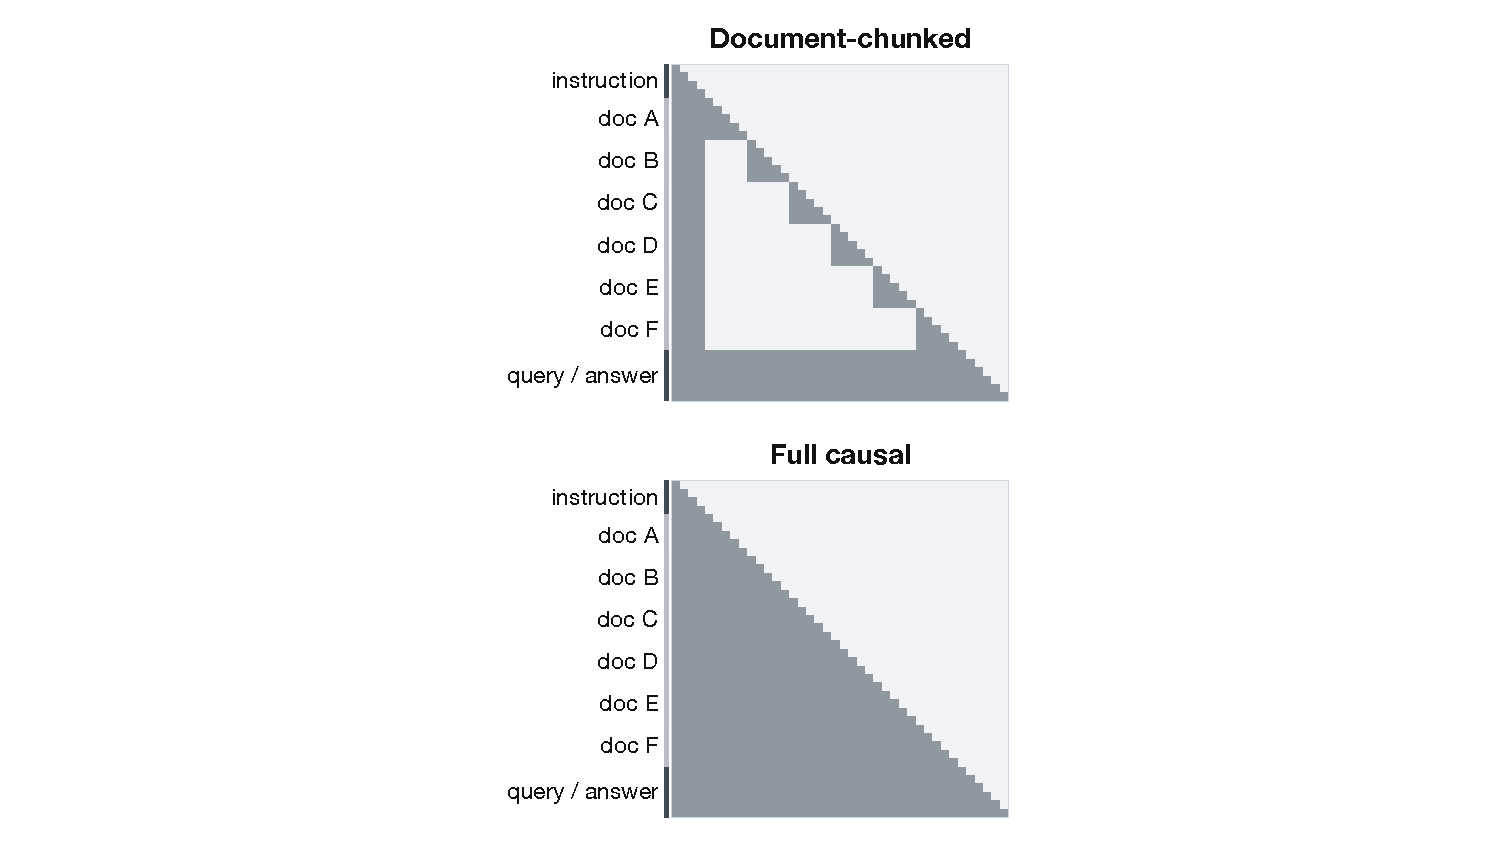
\includegraphics[width=0.45\linewidth, trim=300 30 300 20]{figures/attn_v2.pdf}
    \caption{\textbf{Document-Chunked Attention} Compared to standard full attention, in document-chunked attention documents only attend to themselves.}
    \label{fig:attention_types}
    \vspace{-1em}
\end{wrapfigure}

Due to the prohibitive quadratic cost of \textbf{full attention} (Figure~\ref{fig:attention_types}), attention complexity of transformers has been heavily studied. In one line of work, alternative architectures such as state-space-models (SSMs) \citep{Katharopoulos2020TransformersAR, Gu2023MambaLS} and adjacent approaches like \emph{gated delta net (GDN)} \citep{Yang2024GatedDN} have also enabled linear attention. While this has shown promise, pure-GDN has, even at low-\cname, proven insufficient, and modern language models like Qwen3.5 (CITE) have only mixed, rather than replaced full attention with GDN. For our investigation, we study both hybrid and standard models.

Conversely, particularly for corpus reasoning tasks, \textbf{document-chunked attention} (Figure~\ref{fig:attention_types})---where chunks attend within themselves, save for ``free'' aggregation tokens at the end of context---and adjacent approaches (CITE several) have long been popular, with strong results on common benchmarks and linear (\cmc{N}) complexity \cite{Beltagy2020LongformerTL}. 

We further propose and apply a new trick---\textbf{mask mixing}: during chunked attention training, we mix in a random $p$ percentage of full attention mask training batches into training, and \emph{then use chunked attention for evaluation}. $p=0$ is just chunked attention, and $p=1$ is just full attention training. We find mask-mixing surprisingly beneficial on various tasks (Table~\ref{tab:maskmix}), potentially due to its quadratic train-time attention complexity. While not the focus of this work, we encourage future work to explore it further.

% Corpus \emph{task} complexity provides a framework to understand how task difficulty may scale to larger corpora, but what does this mean for architecture design? We hypothesize that \cname will share a strong relationship with \emph{inference computation}. The most naive case of this is model scale---regardless of the task we'd expect larger models to provide more computation and thus scale better to larger-scale and more complex corpus reasoning tasks than smaller ones. At scale, we posit that attention \emph{complexity} could play an even larger role. \prasannnote{sort of previewing later analysis figures}


% While these methods have enabled comparable performance on certain tasks with much less computation, it's unclear whether this free lunch applies to high-\cname corpus reasoning. In tasks where a task's oracle computation requirements grow rapidly with corpus size, contrary to the typical preference for lower attention complexity, architectures may need as much inference computation as possible to keep up. In fact, even within methods with \cmc{N^2} attention, for example random sparse approaches (TODO cite stuff) (see Figure~\ref{fig:masks} for a naive example), may not have sufficient attention computation for more complex tasks. The interplay of these various computational factors with \cname will be the focus of our empirical investigation. \prasann{Do we need NSA or MoBA experiments? Worst case should try to frame random sparse exp as way to sanity-check that space of things}.

% Given a corpus and method, we can have a separate \emph{inference complexity} indicating how model FLOPs scale with corpus size. Similar to how \cname scales with $N$ oracle operations, method computation, for the models that we investigate, scales via \emph{attention complexity }(e.g. full transformer attention is \cmc{N^2} \prasann{cite attention}). Note that while attention technically scales with token count, assuming constant average document length, $N$ can be used interchangeably to mean token or document count. 

% \prasannnote{Could explain }

% The task-centric notion of \cname is central to our investigation, but how does this interface with \textbf{method} computation? At the heart of our investigation is the hypothesis that, for high \cname tasks, we need attention that's appropriately expressive (Section~\ref{sec:task-def}), but how can we measure attention's expressivity? 

% \prasannnote{expressivity}

% \prasannnote{say that it's potentially tractable, talk about how you control these by modifying masks}

% \prasannnote{make a different O for method comp maybe}

% \prasannnote{attention complexity}


% We vary attention computation on a spectrum of \emph{sparsity} (see Figure~\ref{fig:masks}), where we can control which tokens attend to each other via attention masks. Note that query / answer tokens can always attend to all documents in our settings. One extreme is \textbf{full causal attention}, where every claim token can attend to every preceding claim token in the context---but with \cmc{N^2} computation cost scaled by token count. On the other end is \textbf{document-chunked attention, \cmc{N}}, where individual claims can attend within themselves, but \emph{can't} attend to any other claims---complexity is \cmc{N}, but query / CoT / answer tokens thus must handle searching / composing over claims. In the middle, we test \textbf{random-sparse attention, \cmc{N^2}}, where each claim can attend to a random $N\%$ of other claim tokens, thus being able to get information from other claims (still $N^2$, but with a lower base computation). We base these approaches on a large body of LCLM prior work \cite{Beltagy2020LongformerTL} \prasann{TODO more cite}.


% As such approaches are non-trivial / potentially intractable to set up for \ctc{N^2} tasks, \emph{our investigation will focus on LCLMs}, though chunked attention can be considered a more expressive and end-to-end proxy for such approaches.


% \prasannnote{Hmm I'm thinking about this, maybe we should frame mask mixing as a contribution and put it at the end (can exclude from main multi-task figure)? I think a reviewer might've actually suggested this, TODO will decide based on how universally it helps}

 % \prasann{TODO put description of curriculum mask-mixing here as a paragraph}


% \prasann{TODO figure out which settings use CoT}

